\documentclass[12pt]{article}

\usepackage[a4paper,top=2cm,bottom=2cm,left=2cm,right=2cm,marginparwidth=1.5cm]{geometry}
\usepackage{graphicx}
\usepackage{amssymb}
\usepackage{epstopdf}
\usepackage[german]{babel}
\usepackage[utf8]{inputenc}
\usepackage{pdfpages}
\usepackage{fancyhdr}
\usepackage{amsmath}
\usepackage{tabularx}
\usepackage{makecell}
\usepackage{array}
\usepackage{booktabs}
\usepackage{float}


\DeclareGraphicsRule{.tif}{png}{.png}{`convert #1 `dirname #1`/`basename #1 .tif`.png}

\title{Bericht}
\author{Alisa Pesteritz, Saliha Altan, Wiktoria Cholewa, \\ 
	Dominik Falk, Andreas Kasarinow, Johanna Kleidorfer, \\
	Adrika Narasimhan, Rosina Röckseisen}

\begin{document}

\newpage
\maketitle

\newpage
\pagestyle{fancy}
\fancyhead{}
\fancyhead[L]{Alle}
\section{Einleitung}
\label{einleitung}

\newpage
\pagestyle{fancy}
\fancyhead{}
\fancyhead[L]{Johanna}
\section{Grundlagen}
\label{grundlagen}

\subsection{Biologische Grundlagen}
\label{bio-grundlagen}

\subsubsection{Genexpression und -regulation}

Die im Folgenden analysierten Genexpressionsdaten beschreiben die Aktivität eines Gens und damit, wann und in welcher Intensität ein Gen abgelesen wird. Dies entscheidet über den Phänotyp einer Zelle, denn auch wenn die Zellen eines Organismus dieselbe genetische Information in Form von DNA enthalten, erfüllen sie doch sehr unterschiedliche Funktionen. Die Genexpression folgt dabei dem Zentralen Dogma der Molekularbiologie, bei der Transkription wird die in der DNA kodierte Information in RNA und anschließend mittels der Translation in Proteine überführt \cite{LeeYoung2013}.

Dieser Prozess der Genexpression unterliegt einer zellinternen Genregulation. Dabei binden Transkriptionsfaktoren an regulatorische DNA-Abschnitte wie Promotoren und Enhancer und rekrutieren darüber die RNA-Polymerase, welche das Ablesen des jeweiligen Genabschnitts startet. Je nach gebundenem Transkriptionsfaktor wird die Transkription gehemmt oder aktiviert, es kommt also entweder zum Ablesen oder nicht. Transkriptionsfaktoren sind dabei selbst Proteine, die als Genprodukte anderer Gene entstehen. Je nach Zelltyp, Entwicklungsstadium und äußeren Signalen sind verschiedene Transkriptionsfaktoren vorhanden und aktiv. Diese kaskadierenden Genregulationsnetzwerke erklären, warum trotz identischer DNA in jeder Zelle andere Gene ausgelesen werden \cite{LeeYoung2013}.

Die Feinjustierung der Genexpression umfasst mehrere nachgelagerte Ebenen. Post-transkriptionell wird beispielsweise durch microRNAs oder alternatives Spleißen reguliert, diese Prozesse entscheiden welche und wie viel mRNA für die Translation zur Verfügung steht. Translational wird die Proteinbiosyntheserate kontrolliert, welche bestimmt, wie viele funktionale Proteine aus einer gegebenen mRNA-Menge tatsächlich entstehen. In der post-translationalen Ebene findet schließlich die Proteinmodifikation (z.B. Phosphorylierung, Ubiquitinierung) statt. Eine Abnormalität in einer dieser Kontrollebenen kann zur Fehlregulation der Genexpression und infolgedessen zu Krankheitsbildern führen \cite{LeeYoung2013}.

Die Datenerhebung der möglicherweise dafür verantwortlichen RNA-Mengen erfolgt nach heutigem Stand der Technik meist über das High-Throughput-Verfahren des Next-Generation-Sequencing (RNA-Seq). In Ausnahmefällen werden noch ältere Microarray-Technologien verwendet, diese haben allerdings eine geringere Sensitivität und einen eingeschränkteren dynamischen Messbereich als RNA-Seq \cite{Wang2009}. Der bioinformatische Workflow führt dabei von der RNA-Isolation über das Alignment an ein Referenzgenom bis hin zur Generierung einer rohen Count-Matrix \cite{Kukurba2015}. Diese Matrix bildet das Ergebnis der Sequenzierung ab, sie enthält für jedes Gen (Zeilen) und jede untersuchte Probe oder jeden Patienten (Spalten) die Anzahl der Reads. Ein solches tabellarische Format erwartet auch der CSV-Upload des, in diesem Projekt entwickelten Dashboards (siehe Kap.~\ref{gui}).

Bei diesen Rohdaten kommt es jedoch unweigerlich zu systematischen Verzerrungen, bedingt durch variierende Genlängen und stark schwankende Sequenziertiefen zwischen den einzelnen Probenläufen. Die Sequenziertiefe bezeichnet dabei die Gesamtzahl der in einem Lauf erzeugten Reads für eine Probe und kann zwischen den Proben stark variieren. Ein direkter Vergleich zweier Proben unterschiedlicher Sequenziertiefen würde also fälschlicherweise einen Unterschied in der Genaktivität suggerieren, obwohl dieser lediglich an der Datenmenge liegt. Für eine valide biologische Vergleichbarkeit müssen die Datensätze daher zwingend mathematisch normalisiert werden, bevor sie miteinander verglichen werden können (siehe Kap.~\ref{normalisierung}) \cite{Oshlack2010}.

Die Analyse der Genexpressionsdaten ist vorrangig für die Onkologie von großem Interesse. Dabei wird die Genaktivität quantifiziert und analysiert, wofür das Transkriptom, also die Gesamtheit aller zu einem bestimmten Zeitpunkt in einer Zelle transkribierten RNA-Moleküle, betrachtet werden muss \cite{Conesa2016}. Denn nicht nur das Genom, also die strukturelle DNA und deren Mutationen, ist entscheidend für die Entstehung und das Fortschreiten vieler Krankheitsbilder, sondern maßgeblich auch die zelluläre Aktivität. So lassen sich beispielsweise pathophysiologische Prozesse wie unkontrolliertes Zellwachstum oder die Metastasierung bei strukturell intakten Genen beobachten, wenn diese fehlerhaft reguliert (über- oder unterexprimiert) sind \cite{Vogelstein2013}.

Zu berücksichtigen ist dabei außerdem, dass Genexpression kein synchroner, sondern ein zeitlich gestaffelter, asynchroner Prozess ist. Wird eine Zelle beispielsweise durch einen Wachstumsfaktor oder eine DNA-Schädigung stimuliert, werden nicht alle beteiligten Gene gleichzeitig abgelesen. Zuerst reagieren einzelne, meist regulatorisch wirkende Gene innerhalb weniger Minuten, deren Genprodukte wiederum weitere, nachgeschaltete Zielgene erst zeitversetzt aktivieren \cite{LeeYoung2013}. Eine einzelne RNA-Seq-Messung bildet dabei stets nur eine Momentaufnahme dieses dynamischen Prozesses ab. Zwei Gene, die demselben biologischen Signalweg angehören, müssen in einer solchen Momentaufnahme also nicht zwangsläufig ein gleich starkes Expressionsniveau aufweisen.


\subsubsection{Pathways und die KEGG-Datenbank}

Da viele biologische Prozesse jedoch nicht monogen ablaufen, reicht die Betrachtung einzelner Gene meist nicht für die biologische Interpretierbarkeit. Deshalb müssen funktionell zusammenhängende Gene gemeinsam betrachtet werden, um Muster und Zusammenhänge erkennen zu können. Dementsprechend ist es wichtig die Gene zusammen darzustellen, welche an denselben biologischen Signalwegen beteiligt sind, dies kann durch sogenannte Pathways realisiert werden. Dabei handelt es sich um kuratierte Netzwerke von Genen bzw. Genprodukten, die gemeinsam einen gewissen Signalweg abbilden, wie beispielsweise den einer Signaltransduktion. Die Pathways reduzieren für die Analyse der Daten die Komplexität und erhöhen dabei gleichzeitig die Interpretierbarkeit der Ergebnisse, da sie den funktionalen Kontext liefern \cite{Khatri2012}.

Eine der wichtigsten Referenzdatenbanken, welche hunderte dieser kuratierten Pathways für unterschiedlichste Organismen bereithält, ist die Kyoto Encyclopedia of Genes and Genomes (KEGG) \cite{Kanehisa2023}. KEGG bildet Signalwege, Stoffwechselwege und krankheitsassoziierte Prozesse als standardisierte grafische annotierte Netzwerke ab und beinhaltet pro Pathway die zusammengehörigen Gene. Damit können die Genexpressionsdaten direkt auf die bekannten biologischen Zusammenhänge abgebildet werden. 

Das in diesem Projekt entwickelte Dashboard erlaubt es den Nutzern verschiedenste Pathways der KEGG-Datenbank auszuwählen. Damit lässt sich die Analyse gezielt auf die für einen bestimmten Signalweg relevanten Gene eingrenzen, anstatt anstatt alle in der Count-Matrix enthaltenen Gene gemeinsam betrachten zu müssen. Genaueres zur technischen Implementierung ist in Kapitel~\ref{pathways} zu finden.


\subsection{Medizinische Grundlagen}
\label{medizin-grundlagen}

\subsubsection{Klinische Relevanz der Genexpressionanalyse}

Das entwickelte Tumorboard-Dashboard findet vorrangig im klinischen Kontext, bei der Entwicklung personalisierter Therapiepläne, Anwendung. Ärzte sind hierbei besonders an der Genexpression und deren Regulation interessiert, da herkömmliche histopathologische, also rein visuelle Untersuchungen des Tumorgewebes die molekulare Heterogenität von Tumoren meist nicht vollständig abbilden können \cite{Vogelstein2013}. Denn zwei histologisch identische Tumore können auf molekularer Ebene vollkommen unterschiedliche Aktivitätsprofile aufweisen und entsprechend unterschiedlich auf verschiedene Therapien ansprechen. Diese Informationsebene kommt im klinischen Bereich besonders für die Diagnosen, die Prognoseabschätzung und die Vorhersage der Erfolgschancen bei Therapieansätzen zum Einsatz \cite{NarrandesXu2018}. Beispiele aus der heutigen Zeit für den Einsatz der Genexpressionsdaten sind die Bestimmung des Ursprungsgewebes bei Tumoren unbekannter Herkunft, die Therapieentscheidung bei Brustkrebs sowie die Einschätzung des Rezidivrisikos, also der Wahrscheinlichkeit, dass die Erkrankung nach erfolgreicher Genesung erneut auftritt \cite{NarrandesXu2018}.

\subsubsection{Das Molekulare Tumorboard}

Das Molekulare Tumorboard (MTB) ist eine interdisziplinäre Expertenkonferenz, in der für besondere Krankheitsbilder oder spezielle Verläufe individualisierte Therapiepläne entwickelt werden. Hier dienen die genomischen und transkriptomischen Profile der Entscheidungsfindung \cite{Tamborero2020}.

\subsubsection{Das Dashboard als Clinical Decision Support System}

Das Dashboard fungiert hierbei als interaktives Clinical Decision Support System (CDSS) \cite{Tamborero2020}. Es bietet mit der Heatmap und den Dendrogrammen eine gemeinsame, leicht verständliche, visuell dargestellte Diskussionsgrundlage für die beteiligten Experten. Es erlaubt einem interdisziplinären Kollektiv aus Onkologen, Pathologen, Chirurgen und Bioinformatikern die medizinischen Analysen ohne Programmierkenntnisse in Echtzeit über eine grafische Benutzeroberfläche zu steuern und anschließend gemeinsam darüber zu beraten. 

Das Ziel des interdisziplinären Gremiums besteht dementsprechend darin, die genomischen und transkriptomischen Profile der Patienten mithilfe des CDSS gemeinschaftlich zu evaluieren und mit den daraus generierten Informationen eine individuelle Therapieempfehlung auszuarbeiten. Denn wichtige und weitreichende Therapieentscheidungen können nicht von einem einzelnen Arzt isoliert verantwortet werden \cite{Mosele2020}. Studien belegen, dass diese Art der computergestützten Therapiewahl die Behandlungsergebnisse maßgeblich verbessern kann \cite{Horak2021}. Durch die Anpassungsmöglichkeiten, wie die Auswahl spezifischer biologischer Pathways, die Modifikation der Normalisierungsverfahren, die Wahl des Cluster-Algorithmus (z.\,B. Single, Average und Complete Linkage) und der farblichen Darstellung kann das Dashboard zum zentralen Visualisierungsmedium in der Konferenz werden. Das ermöglicht den Ärzten, Hypothesen direkt während der Sitzung gemeinsam zu prüfen, molekulare Muster im Kollektiv zu interpretieren und so die bestmögliche personalisierte Therapieempfehlung für die Patienten auszuarbeiten \cite{PereraBel2018}.

\subsubsection{Informatische Grundlagen}
\label{info-grundlagen}
Was ist eine explorative Datenanalyse?

Was ist Clustering?


\section{Arbeitseinteilung (oder sowas)}
\label{arbeitseinteilung}
% TODO: wer hat was gemacht und warum?
% Datenfluss (von Johanna) einfügen? (oder zumindest beschreiben?)

% ----------------------------------------------------------------------------------------------
\newpage
\pagestyle{fancy}
\fancyhead{}
\fancyhead[L]{Alisa}
\section{Pathways und Dateneinlesen}
\label{pathways}

Die Tabelle zeigt, wie groß der Arbeitsaufwand pro Unteraufgabe ausgefallen ist.
\begin{table}[h!]
	\centering
	\begin{tabular}{p{8cm}|l|l}
		Aufgabe & Zuständig & Arbeitsaufwand \\ 
		\hline
		Recherche zu Pathways und Extraktion der Daten von KEGG & Alisa & 5 Stunden \\
		Datenbank entwerfen und aufsetzen & Alisa & 7 Stunden \\ 
		Funktionen: Prozessierung, Datenbankabfragen und Integration & Alisa & 17 Stunden \\ 
		Datensätze bearbeiten & Alisa & 5 Stunden \\          
		Besprechungstermine & Alle & 19,5 Stunden \\    
		Berichterstellung & Alisa & 5 Stunden \\    
	\end{tabular}
\end{table}

\noindent Der Bereich Pathways und Dateneinlesen untergliedert sich in mehrere Teilbereiche, welche im Folgenden näher erläutert werden.

\subsection{Datenbeschaffung}
Das zentrale Ziel des Aufgabenbereiches war die semantische Datenintegration biologischer Genexpressionsdatensätze. Konkret sollte es möglich sein, aus einem größeren Genexpressionsdatensatz, gezielt die Gene herauszufiltern, die den vom Nutzer ausgewählten biologischen Pathways zugeordnet sind.
Voraussetzung dafür ist eine strukturelle Grundlage für die Verknüpfung der Pathways mit ihren zugehörigen Genen. Dafür wurde die KEGG-Datenbank verwendet, welche im Abschnitt \ref{bio-grundlagen} zusammen mit der Funktion der Pathways näher erläutert wird. KEGG stellt eine öffentliche REST-API-Schnittstelle bereit, über die die folgende Informationen abgerufen und als CSV-Dateien gespeichert wurden: 
\begin{itemize}
	\item Pathway-Liste: Alle menschlichen Pathways mit ihrer KEGG ID und ihrem Namen. Abgerufen über \texttt{https://\allowbreak rest.\allowbreak kegg.\allowbreak jp/\allowbreak list/\allowbreak pathway/\allowbreak hsa}.
	\item Gen-Pathway Verknüpfungen: Die Zuordnung von Genen zu ihren entsprechenden Pathways. Abgerufen über \texttt{https://\allowbreak rest.\allowbreak kegg.\allowbreak jp/\allowbreak link/\allowbreak pathway/\allowbreak hsa}.
\end{itemize}
\noindent Die CSV-Dateien wurden anschließend in R bereinigt. Präfixe wie \texttt{path:} und \texttt{Homo sapiens} wurden entfernt, um nur die relevanten Informationen abzubilden. 

\noindent Da über die KEGG-API nur Entrez IDs und keine Gennamen bereitgestellt wurden, mussten die zugehörigen Gennamen nachträglich gemappt werden. Hierzu wurden über die Annotationsbibliothek \texttt{org.Hs.eg.db} gezielt die Entrez IDs mit den entsprechenden Gennamen verknüpft, die in den abgerufenen Pathways enthalten sind.

\subsection{Aufbau der lokalen SQLite Datenbank}
Auf Basis der KEGG-Daten sowie der Zuordnung von Entrez IDs zu Gennamen wurde eine lokale SQLite-Datenbank \texttt{"GeneDatabase.sqlite"} aufgebaut. Diese dient als semantisches Bindeglied zwischen den Genexpressionsdatensätzen und den Pathways. Die Entscheidung für eine relationale Datenbank fiel aufgrund des deutlich effizienteren Datenzugriffs im Vergleich zu CSV- oder Excel-Dateien. Die daraus resultierende Datenbank besteht aus drei Tabellen: 
\begin{itemize}
	\item Gene: Enthält die Entrez ID als Primärschlüssel, den vollständigen Gennamen sowie das Gensymbol
	\item Pathway: Enthält die KEGG- Pathway ID und den Namen des Pathways.
	\item Lookup\_Gene\_Pathway: Stellt eine N:M Relation zwischen Genen und Pathways dar.
\end{itemize}

\begin{figure}[h!]
	\centering
	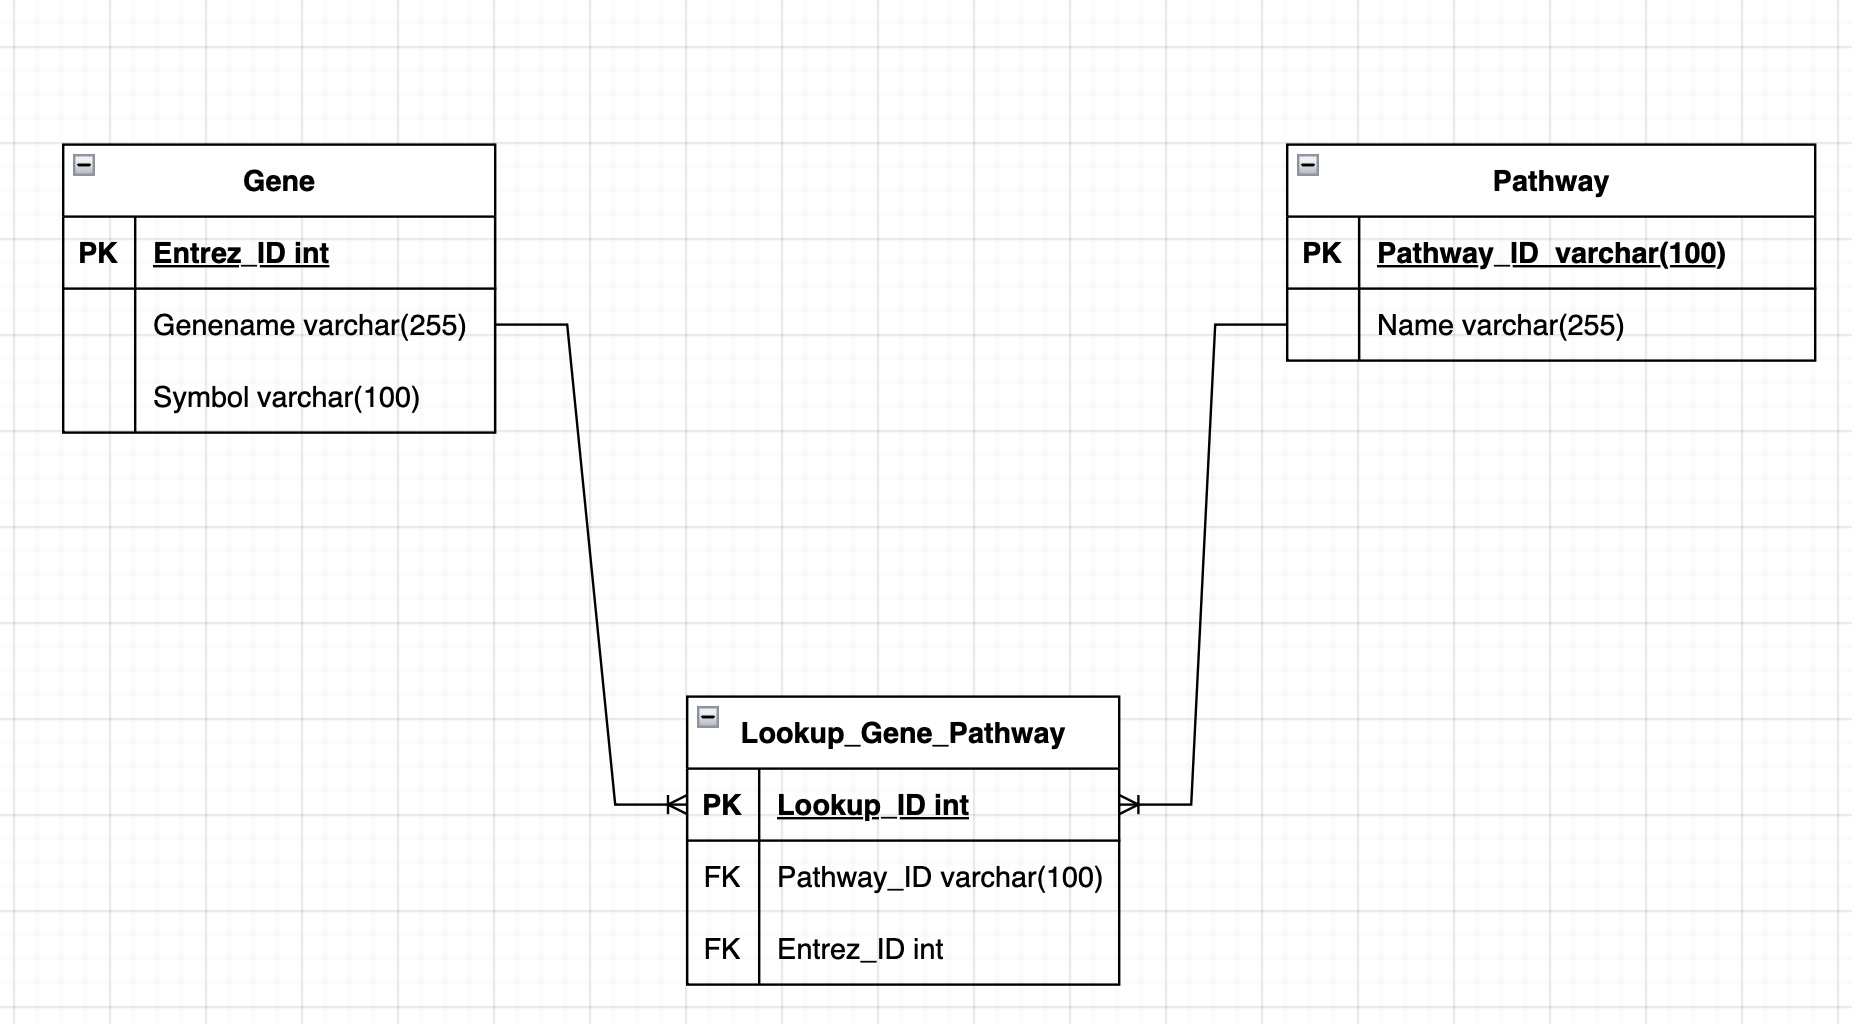
\includegraphics[width=0.7\textwidth]{ERM_Modell.jpg}
	\caption{Eigene Darstellung: ERM Modell zum Aufbau der Datenbank}
\end{figure}

\subsection{Funktionen zur Datenvorverarbeitung und Datenintegration}

\noindent Die gesamte Programmlogik ist modular aufgebaut und gliedert sich funktional in vier zentrale Aufgabenbereiche: Datenvorverarbeitung zur Metadaten-Trennung, Coverage Analyse, Datenbankabfragen sowie die finale Datenintegration.
Es existieren zwei spezialisierte Vorverarbeitungsfunktionen, die je nach Datentyp der ersten Spalte des Datensatzes aufgerufen werden: \texttt{preprocess\_\allowbreak dataset\_\allowbreak meta()} extrahiert numerische Entrez IDs, während \texttt{preprocess\_\allowbreak dataset\_\allowbreak meta\_\allowbreak gennames()} genutzt wird, wenn Gennamen als \texttt{character} vorliegen. Beide Funktionen implementieren die Trennung von Messwerten und Metadaten über die Identifikation des Präfixes (\texttt{Meta\_}). Dies ermöglicht es die Metainformationen separat von den eigentlichen Genexpressionsdaten zu speichern, sodass andere Teammitglieder für ihre Teilaufgaben direkt darauf zugreifen können.

\subsubsection{Pathway Coverage}

\noindent Bevor die eigentliche Datenintegration durchgeführt wird, kann mit der Funktion \texttt{analyze\_\allowbreak pathways\_\allowbreak coverage()} geprüft werden, wie gut die vom User ausgewählten Pathways durch den hochgeladenen Datensatz abgedeckt werden. Für jeden gewählten Pathway wird anhand einer Datenbankabfrage ermittelt, wie viele der in der Datenbank hinterlegten Gene im Datensatz vorhanden sind und wie viele fehlen. Die Funktion gibt eine Matrix mit den Spalten Gesamtanzahl, gefundene Gene, fehlende Gene sowie der prozentualen Abdeckung (Coverage) zurück. Diese Funktion dient als wichtige Entscheidungsgrundlage, um die Aussagekraft der nachfolgenden Analysen zu bewerten. Bei einer unzureichenden Abdeckung erhält der Nutzer somit die Möglichkeit, die Pathway Auswahl frühzeitig zu optimieren.

\subsubsection{Datenintegration}
\label{subsec:semantische_integration}

\noindent Die Kernfunktion \texttt{run\_data\_integration()} verbindet alle Hilfsfunktionen und führt die semantische Filterung der Daten nach ausgewählten Pathways durch. Der Ablauf ist wie folgt:

\begin{itemize}
	\item Der Datensatz wird anhand des Datentyps der ersten Spalte mit der passenden Funktion vorverarbeitet und von den Metadaten separiert.
	\item Über Datenbankabfragen werden alle relevanten Gene ermittelt, die den vom Nutzer gewählten Pathways zugeordnet sind. Es werden sowohl die IDs als auch die zugehörigen Gennamen in Vektoren gespeichert.
	\item Mittels der Funktion \texttt{extract\_relevant\_genes()} wird der Datensatz auf diese Gene reduziert. Werden keine Übereinstimmungen gefunden, bricht der Prozess mit einer Fehlermeldung ab. 
	\item Die Funktion \texttt{rename\_duplikate\_genes()} behandelt mehrfach vorhandene IDs und macht sie über ein Suffix eindeutig (z.\,B. \texttt{"51\_1"}, \texttt{"51\_2"}). Durch diese Eindeutigkeit können die IDs nun als Zeilennamen verwendet werden.
	\item Als Ergebnis wird eine benannte Liste zurückgegeben, die den gefilterten Datensatz, die Metadaten, den Genvektor sowie die zugehörigen Gennamen enthält.
\end{itemize}

\subsection{Datensätze}

\noindent Zum Testen der implementierten Funktionen wurden vier Genexpressions-Datensätze bereitgestellt. Zwei dieser Datensätze stammen aus dem TCGA-Register. 

\noindent The Cancer Genome Atlas (TCGA) ist ein großes, öffentliches Forschungsprogramm, welches umfassende genomische Daten und klinische Metadaten von über 33 verschiedenen Krebsarten bereitstellt \cite{CGARN2013}. 

\noindent Zwei der für dieses Projekt verwendeten Testdatensätze stammen aus diesem Programm: 
\begin{itemize}
	\item \textbf{colon\_vs\_pancreas\_meta.csv}: Datensatz, der Proben von Darm- und Bauchspeicheldrüsenkrebs vergleicht.
	\item \textbf{TCGA\_kidney\_unnormalized\_meta.csv}: Datensatz, der die drei Nierenkrebs-Unterarten: papilläres, chromophobes und klarzelliges Nierenzellkarzinom enthält.
\end{itemize}
\noindent Ein weiterer zur Verfügung gestellter Datensatz ist der Golub-Datensatz: \textbf{GOLUB\_microarray.csv}. Dieser enthält Genexpressionsdaten, die genutzt wurden, um Patienten mit zwei verschiedenen Arten von Blutkrebs zu klassifizieren: der akuten myeloischen Leukämie und der akuten lymphatischen Leukämie \cite{Golub1999}. 

\noindent Der letzte zur Verfügung gestellte Datensatz ist der SHIPP-Datensatz: \textbf{SHIPP\_microarray.csv}. Dieser enthält zwei Formen von Non-Hodgkin-Lymphomen: das diffuse großzellige B-Zell-Lymphom und das follikuläre Lymphom \cite{Shipp2002}.

\noindent Die Datensätze wurden nach einem einheitlichen Schema aufbereitet und für alle Teammitglieder bereitgestellt: Während die erste Spalte immer die numerischen Entrez IDs oder Gennamen enthält, repräsentieren die darauffolgenden Spalten die einzelnen Patientenproben. Zur Erweiterung der Metadaten wurden für alle Datensätze zufällige Werte für Alter und Geschlecht generiert. Um die Metadaten sauber von den eigentlichen Genexpressionsdaten zu trennen, wurden diese einheitlich mit dem Präfix \texttt{Meta\_} versehen.

% ----------------------------------------------------------------------------------------------
\newpage
\pagestyle{fancy}
\fancyhead{}
\fancyhead[L]{Rosina und Wiktoria}
\section{Clusterverfahren}

\subsection{Arbeitsverteilung}
\label{cluster-arbeitsverteilung}
Der Bereich der Clusteranalyse unterteilt sich in mehrere Unteraufgaben. Zunächst wurden die Daten auf die Weiterverarbeitung vorbereitet mit Hilfe einer Preprocessing-Funktion. Der Datensatz wurde daraufhin normalisiert, wobei unterschiedliche Normalisierungsfunktionen zur Auswahl standen. Aus dem normalisierten Datensatz wurde eine Distanzmatrix berechnet und anschließend ein Linkage-Verfahren angewendet. Dementsprechend mussten neben der Preprocessing-Funktion auch die Normalisierungs-, Distanz- und Linkage-Funktionen implementiert werden. 

Die folgende Tabelle zeigt, welche Aufgaben von wem übernommen wurden und wie groß der Arbeitsaufwand war.

\begin{table}[h!]
	\begin{tabular}{l|l|l}
		Aufgabe                       & Zuständig & Arbeitsaufwand \\ 
		\hline
		Datenvorbereitung             & Rosina    & 6 Stunden        \\
		Normalisierungsfunktionen     & Rosina    & 6 Stunden           \\ 
		Testen                        & Rosina    & 14 Stunden        \\
		Recherche                     & Rosina    & 5,5 Stunden        \\
		Bericht schreiben             & Rosina    & 10 Stunden        \\
		Besprechungen                 & Rosina    & 19,5 Stunden        \\
		Complete-Linkage              & Rosina    & 30 Minuten        \\ 
		Average-Linkage               & Rosina    & 1 Stunde         \\ 
		Recherche zu Distanzfunktinen 						& Wiktoria  & 3 Stunden \\
		Programmieren der Distanzfunktionen      			& Wiktoria  & 7 Stunden \\ 
		Recherche zu Linkagefunktionen 						& Wiktoria  & 4 Stunden \\
		Linkagefunktionen nach Lance-Williams   			& Wiktoria  & 12 Stunden   \\
		Testen (inkl. GUI- und Visualisierungsfunktionen)   & Wiktoria  & 25 Stunden  \\ 
		Besprechungen 				 						& Wiktoria  & 19,5 Stunden  \\
		Protokollvor- und Nachbereitung 					& Wiktoria  & 3 Stunden \\
		Berichterstellung (eigenes Kapitel)					& Wiktoria  & 10 Stunden \\
		Bericht zusammenfügen und Korrektur                 & Wiktoria  & 3 Stunden \\
		Folien zusammenfügen und Korrektur 					& Wiktoria  & 1 Stunde \\
		Repository-Pflege 									& Wiktoria  & 3 Stunden \\
		Erstellen einer Library 							& Wiktoria  & NOCH OFFEN \\
	\end{tabular}
\end{table}

\subsection{Allgemeines Vorgehen}
\label{allgemein-clusterung}

Nach der Filterung der Genexpressionsdaten müssen sie für die anschließende Clusteranalyse vorbereitet werden. Rohdaten können fehlende Werte, unterschiedliche Wertebereiche oder andere Eigenschaften aufweisen, die die Qualität der Clusterbildung negativ beeinflussen. Eine sorgfältige Vorverarbeitung stellt daher sicher, dass die Daten in einer geeigneten Form für die Distanzberechnung und die Clusteranalyse vorliegen.

Die Vorverarbeitung besteht aus zwei Schritten. Zunächst werden die Daten auf Vollständigkeit und Gültigkeit überprüft sowie fehlende Werte behandelt. Anschließend erfolgt optional eine Normalisierung der Daten. Je nach gewählter Methode werden die Expressionswerte transformiert und skaliert um Unterschiede in den Wertebereichen zwischen den Genen zu reduzieren und die Vergleichbarkeit der Expressionsprofile zu verbessern. Dadurch wird eine zuverlässigere Grundlage für die nachfolgenden Clustering-Verfahren geschaffen.

Anfangs stellt jedes Element des Datensatzes (jede Beobachtung; dies bezieht sich auf die Gene, sowie auf die Patienten) ein eigenes Cluster dar. In jedem Schritt werden zwei Cluster zusammengefasst, bis schließlich alle Elemente in einem Cluster vereint sind. Das Zusammenfassen erfolgt mit einem bestimmten Linkage-Verfahren und basiert auf den Distanzen der Cluster zueinander. Zu diesem Zweck wird zunächst eine Distanzmatrix erstellt, die für alle Paare aus Elementen des Datensatzes die entsprechende Distanz enthält. Nach jedem Schritt werden die Distanzen für das neue Cluster aktualisiert. Je nach gewählten Linkage-Verfahren entstehen so unterschiedliche Aktualisierungen und damit auch unterschiedliche Cluster.

\newpage
\pagestyle{fancy}
\fancyhead{}
\fancyhead[L]{Rosina}

\subsection{Datenvorbereitung}
\label{datenvorbereitung}

Vor der Normalisierung wird der Datensatz auf seine Eignung für die weitere Verarbeitung überprüft. Dies geschieht in der Funktion \texttt{prepare\_data}, welches auffindbar im Github-Projekt unter \texttt{R/clustering/prepare\_data.R} ist. Ziel dieser Funktion ist es, fehlerhafte oder unvollständige Eingabedaten frühzeitig zu erkennen und eine konsistente Datenstruktur für die anschließende Clusteranalyse sicherzustellen.

Als Erstes wird überprüft, ob der übergebene Datensatz leer ist oder keine Zeilen beziehungsweise Spalten enthält. Darüber hinaus wird kontrolliert, ob mindestens zwei Zeilen vorhanden sind, da eine Clusteranalyse mehrere Beobachtungen voraussetzt.
Anschließend erfolgt eine Plausibilitätsprüfung der Werte. Falls der Datensatz nicht bereits als normalisiert gekennzeichnet wurde, wird überprüft, ob Werte kleiner als $-1$ enthalten sind. Solche Werte können darauf hinweisen, dass die Daten bereits transformiert oder skaliert wurden und eine erneute Normalisierung ungeeignet wäre. In diesem Fall wird die Verarbeitung mit einer entsprechenden Fehlermeldung abgebrochen.
Für die weitere Verarbeitung wird der Datensatz anschließend in eine Matrix umgewandelt. Anschließend wird der ganze Inhalt zu numerischen Werten konvertiert. Dies stellt sicher, dass berechenbare Zahlen in der Matrix vorhanden sind. Nicht-numerische Werte, wie Buchstaben, werden dadurch zu fehlenden Einträgen (\texttt{NA}) gewandelt. So können sie in der darauffolgenden NA-Behandlung mit entfernt werden.
Der nächste Bestandteil der Datenvorbereitung ist die Behandlung fehlender Werte. Enthält eine Zeile fehlende Einträge, wird zunächst überprüft, ob mindestens ein gültiger numerischer Wert vorhanden ist. Ist dies der Fall, werden die fehlenden Werte, sofern welche in der Zeile vorhanden sind, durch den Mittelwert der numerischen Werte derselben Zeile ersetzt. Auf diese Weise bleiben möglichst viele Informationen erhalten und die NA-Werte werden ersetzt. Enthält eine Zeile ausschließlich fehlende Werte, wird die Verarbeitung abgebrochen, da keine Mittelwertberechnung möglich ist.
Abschließend wird der Datensatz auf unendliche Werte (\texttt{Inf} beziehungsweise \texttt{-Inf}) überprüft. Da solche Werte bei den nachfolgenden Berechnungen zu Fehlern führen würden, wird die Verarbeitung in diesem Fall ebenfalls beendet. Nach Abschluss aller Prüfungen liegt ein vollständiger numerischer Datensatz vor, der für die anschließende Normalisierung und Clusteranalyse verwendet werden kann.

Während der Entwicklung dieser Funktion traten keine größeren Schwierigkeiten auf. Der Entwicklungsaufwand betrug etwa sechs Stunden, während die anschließende Testphase ungefähr vier Stunden in Anspruch nahm. Eine Besonderheit beim Testen der Funktion bestand darin, dass für bestimmte Fehlerfälle eigene, kleine Testdatensätze erstellt werden mussten. Dadurch konnten spezifische Fehler gezielt produziert und überprüft werden, da nicht alle möglichen Fehlerzustände regelmäßig in realen Datensätzen auftreten. Insbesondere die Behandlung von fehlenden Werten (NA-Werten) erforderte eine ausführliche Abstimmung. Hierzu wurde eine längere Zeitspanne einer Besprechung in Anspruch genommen, um festzulegen, unter welchen Bedingungen eine Fehlerbehandlung erfolgen soll und welche Vorgehensweise für die verschiedenen Fälle angemessen ist.

\subsection{Normalisierung}
\label{normalisierung}

Nach der Datenvorbereitung kann der Datensatz optional normalisiert werden. 

Ziel der Normalisierung ist es, den Einfluss technischer Störfaktoren und systematischer Fehler auf die Messdaten zu reduzieren, sodass möglichst ausschließlich die biologische Variabilität der Genexpression erhalten bleibt. Solche unerwünschten Variationen können beispielsweise durch Unterschiede bei der Probenvorbereitung, leichte Schwankungen der Umgebungsbedingungen, den Abbau von Probenmaterial oder technische Einflüsse der verwendeten Messinstrumente entstehen. Generell sind diese Störquellen häufig weder direkt messbar noch exakt quantifizierbar, deswegen stellt ihre Korrektur eine besondere Herausforderung dar \cite{Dubois2022}. 

Eine geeignete Normalisierung trägt daher wesentlich dazu bei, die Vergleichbarkeit der Daten zu verbessern und die Grundlage für eine zuverlässige Clusteranalyse zu schaffen. Für die in diesem Projekt entwickelte Funktion \texttt{normalization} stehen acht verschiedene Normalisierungsmethoden zur Verfügung, die nach dem belieben des Users ausgewählt werden können. Sie ist auffindbar im Projekt unter dem Pfad \texttt{R/clustering/normalization\_methods.R}. 

\subsubsection{Keine Normalisierung}
\label{Keine Normalisierung}

Bei dieser Methode werden die Daten unverändert weitergegeben. Sie eignet sich für Datensätze, die bereits vorverarbeitet oder mit einem externen Verfahren normalisiert wurden. Somit können auch normalisierte Datensätze visualisiert werden.

\subsubsection{Nur Logarithmierung}
\label{Nur Logarithmierung}

In dieser Variante wird ausschließlich die Logarithmierung durchgeführt.
Dies geschieht indem auf alle Expressionswerte nur eine Logarithmierung zur Basis 2 angewendet. Sie hilft den Dynamikbereich als auch die Schiefe der Verteilung zu reduzieren und führt so zu einer stärkeren Symmetrie, sowie nähert die Daten an eine Normalverteilung an. Dadurch erfüllen die Daten die Annahmen statistischer Analysen besser. Um Probleme mit Null- oder sehr kleinen Werten zu vermeiden, wird vor der Anwendung des Logarithmus üblicherweise eine kleine Konstante zu jedem Wert addiert \cite{Deng2025}. Dies wurde in dieser Funktion auch durchgeführt mit einer Addierung von 1. Die Formel des Logarithmus ist wie folgt:

\[x_1'=\log_2(x_1+1)\]

Durch das Logarithmieren werden große Expressionswerte abgeschwächt, während die absoluten Unterschiede zwischen den Genen weitgehend erhalten bleiben \cite{Durbin2002}. In dieser Methode erfolgt keine zusätzliche Skalierung der Daten. Die reine Log-Transformation ist sinnvoll, wenn der Nutzer die Wertekompression benötigt, aber die ursprüngliche Struktur der Daten möglichst unverändert beibehalten möchte. Alle darauffolgenden Logarithmen werden genau wie hier beschrieben durchgeführt.

\subsubsection{Z-Score-Normalisierung}
\label{Z-Score-Normalisierung}

\paragraph{Variante mit Logarithmierung}

Diese Methode startet mit dem logarithmieren der Daten wie in \ref{Nur Logarithmierung} beschrieben.
Anschließend erfolgt für jede Genzeile eine Z-Score-Normalisierung. Die Z-Score-Transformation ist eine weit verbreitete Normalisierungsmethode, bei der Merkmale (Gene) so skaliert werden, dass sie einen Mittelwert von 0 und eine Standardabweichung von 1 aufweisen. Für jedes Gen wird zunächst der Mittelwert ($\mu$) und die Standardabweichung ($\sigma$) über alle Proben hinweg berechnet\cite{Deng2025}. Jeder Wert ($x$) mithilfe der folgenden Formel standardisiert:

\[z_i=\frac{x_1'-\mu}{\sigma}\]

Diese Transformation ermöglicht es, unterschiedliche Merkmale auf eine vergleichbare Skala zu bringen\cite{Deng2025}. Der Nachteil ist, dass sie sensibel gegenüber Ausreißer ist, was zum Teil durch den Logarithmus unterbinden werden kann. Im eigentlichen R Code wird diese Formel mit der \texttt{scale}-Funktion durchgeführt. Da die Funktion spaltenweise arbeitet, wird der Datensatz zunächst transponiert, verarbeitet und abschließend erneut transponiert, um die ursprüngliche Ausrichtung wiederherzustellen.

\paragraph{Variante ohne Logarithmierung}

In dieser Methode wird ausschließlich die Z-Score Normalisierung durchgeführt. Im Gegensatz zur vorherigen beschriebenen Variante erfolgt keine vorherige Logarithmierung der Expressionswerte. Dadurch werden die ursprünglichen Expressionswerte direkt standardisiert.

Diese Variante eignet sich insbesondere für Datensätze, die bereits logarithmiert wurden oder bei denen bewusst auf eine zusätzliche Logarithmierung verzichtet werden soll.

\subsubsection{Median-Zentrierung}
\label{Median-Zentrierung}

\paragraph{Variante mit Logarithmierung}
Auch in dieser Methode wird zunächst die Logarithmierung durchgeführt (siehe \ref{Nur Logarithmierung}). Anschließend wird jede Genzeile um ihren Median zentriert und mithilfe ihrer Spannweite skaliert. Das Ziel der Median-Zentrierung besteht darin, die Daten auf den Median der Verteilung jeder Probe zu zentrieren. Im Allgemeinen wird die Zentrierung anhand des Medians gegenüber dem Mittelwert bevorzugt, da der Median robuster gegenüber Ausreißern ist \cite{Dubois2022}. Der vollständige Normalisierungsprozess wird mit dieser Formel durchgeführt:

\[x_i''=\frac{x_i'-\mathrm{Median}(x')}{\max(x')-\min(x')+\varepsilon}\]

Sie ist entstanden aus der Kombination der Median-Zentrierung und der Range-Skalierung.
Die Formel der Median-Zentrierung ist nach \cite{Dubois2022}: 

\[x_i''={x_i'-\mathrm{Median}(x')}\] 

Bei der Range-Skalierung werden die zentrierten Werte durch die Spannweite, also die Differenz zwischen dem Maximum und Minimum einer Genzeile, dividiert. Dadurch werden Unterschiede in den Wertebereichen der Gene reduziert, sodass alle Gene unabhängig von ihrer ursprünglichen Variabilität einen vergleichbaren Einfluss auf die nachfolgende Analyse besitzen. Da die Spannweite den biologischen Variationsbereich der Daten repräsentiert, orientiert sich die Skalierung an diesem biologischen Wertebereich \cite{Berg2006}. Dargestellt wird es durch diese Formel nach \cite{Berg2006}:

\[x_{ij}^{*}=\frac{x_{ij}-\bar{x}_{i}}{x_{i,\max}-x_{i,\min}}\] 

Das $\varepsilon$ in der vollständigen Formel wird definiert mit $\varepsilon = 1e^{-8}$ und ist eine kleine Konstante, die die Teilung durch Null verhindert.
Ein Nachteil der Range-Skalierung besteht jedoch darin, dass die Spannweite ausschließlich auf den beiden Extremwerten basiert und daher empfindlich gegenüber Ausreißern ist\cite{Berg2006}. Allerdings wird dieser Schwäche zum Teil durch die Median-Zentrierung entgegengewirkt. 

\paragraph{Variante ohne Logarithmierung}

In dieser Methode wird nur die oben beschriebene Median-Zentrierung durchgeführt, während das Logarithmieren ausgelassen wird. Wie schon bereits erklärt ist dies von besonderem Nutzen, wenn die Originalstruktur des Datensatzes von großer Bedeutung, oder der Datensatz schon vorbereitet worden ist.

\subsubsection{MAD-Normalisierung}
\label{MAD-Normalisierung}

\paragraph{Variante mit Logarithmierung}

Diese Methode verwendet ebenfalls zunächst die Logarithmierung(siehe \ref{Nur Logarithmierung}). Anschließend erfolgt eine robuste Skalierung mithilfe der Median Absolute Deviation (MAD):

\[x_i''=\frac{x_i'-\mathrm{Median}(x')}{\mathrm{MAD}(x')+\varepsilon}\]

Dabei bezeichnet

\[\mathrm{MAD}(x)=\mathrm{Median}\left(\left|x-\mathrm{Median}(x)\right|\right)\]

die Median Absolute Deviation. $\varepsilon= 1e-8$ ist erneut eine kleine Konstante, die eine Division durch Null verhindert.
Anstelle der Standardabweichung wird die Median Absolute Deviation (MAD) als robustes Maß für die Variabilität verwendet. Sie entspricht dem Median der absoluten Abweichungen aller Beobachtungen vom Stichprobenmedian \cite{Schmidt}.

Im Vergleich zur Standardabweichung ist MAD deutlich robuster gegenüber Ausreißern und eignet sich daher insbesondere für Datensätze mit einzelnen extremen Expressionswerten \cite{Kappal2019}.

\paragraph{Variante ohne Logarithmierung}

Diese Methode entspricht der im vorherigen Paragraph beschriebenen MAD-Normalisierung, jedoch ohne vorherige Logarithmierung. Die ursprünglichen Expressionswerte werden direkt anhand der Median Absolute Deviation (MAD) skaliert. Diese hat vor allem Nutzen, wenn Reduktion der Verteilung im Datensatz nicht nötig ist und nur der Normalisierungseffekt benötigt wird.

\subsubsection{Herausforderungen bei der Implementierung}
\label{herausforderung-rosina}

Der gesamte Programmieraufwand für die Funktion \texttt{normalization} betrug etwa sechs Stunden. In dieser Zeit wurden sowohl die bestehende Struktur überarbeitet als auch neue Normalisierungsmethoden implementiert. Die eigentliche Implementierung der Funktion erfolgte vergleichsweise zügig. Deutlich zeitintensiver war hingegen das Testen, welches insgesamt etwa zehn Stunden in Anspruch nahm.

Während der Testphase trat bei einem von einem weiteren Tester verwendeten Datensatz ein Fehler auf, dessen Ursache zunächst unklar war. Nach eingehender Analyse stellte sich heraus, dass der Datensatz bereits vorab normalisiert worden war. Zu diesem Zeitpunkt bot das Programm jedoch keine Möglichkeit, bereits vorbereitete Datensätze korrekt zu verarbeiten oder dem Benutzer explizit die Auswahl eines vorab normalisierten Datensatzes zu ermöglichen. Aus diesem Grund wurden entsprechende Optionen für den Benutzer ergänzt sowie zusätzliche Fehlerbehandlungen implementiert.

In der Endphase des Projekts wurde außerdem festgestellt, dass das Clustering beziehungsweise die Darstellung der Cluster nicht korrekt funktionierte. Daraufhin wurde die gesamte Normalisierungsfunktion erneut überprüft und ausführlich getestet. Gleichzeitig wurde der Datensatz, der den Fehler besonders deutlich sichtbar machte, nochmals analysiert. Dabei konnte die eigentliche Fehlerursache identifiziert und behoben werden. Im Zuge dieser Überarbeitung fiel zudem die Entscheidung, den Funktionsumfang zu erweitern und zusätzlich Normalisierungsmethoden ohne vorgeschaltete Logarithmierung zu implementieren.

Einen weiteren unerwartet hohen Zeitaufwand verursachte die Recherche geeigneter Normalisierungsmethoden (5,5 Stunden). Zwar wird in wissenschaftlichen Veröffentlichungen häufig angegeben, dass Verfahren wie beispielsweise die Z-Score-Normalisierung verwendet wurden, jedoch fehlen oftmals detaillierte Beschreibungen der konkreten Implementierung oder eine Begründung für die Wahl der jeweiligen Methode.

% ----------------------------------------------------------------------------------------------
\newpage
\pagestyle{fancy}
\fancyhead{}
\fancyhead[L]{Wiktoria}

\subsection{Berechnung der Distanzmatrix}
\label{distanzfunktionen}
Für das Zusammenfügen der Cluster muss zunächst bestimmt werden, wie ähnlich, bzw. nah diese zueinander sind. Da es sich bei den in diesem Projekt verwendeten Genexpressionsdaten um kontinuierliche Daten handelt, wird ihre Nähe mit Hilfe von Distanzmaßen bestimmt. Für ein Distanzmaß $\delta_{ij}$ muss die Dreiecksungleichung gelten, d.h. für drei Elemente $i$, $j$ und $m$:
 
\[ \delta_{ij} + \delta_{im} \ge \delta_{jm} \]

Durch Berechnen der zeilenweisen Distanzen  \( \delta_{ij} \), für welche diese Bedingung gilt, entsteht eine symmetrische Distanzmatrix \( \mathbf{D}\), wobei \( \delta_{ii}  = 0\) für alle \( i \) gilt \cite{Everitt2011}. Es muss sowohl eine Distanzmatrix für die Gene als auch für die Patienten berechnet werden. Im zweiten Fall wird der Datensatz zunächst transponiert, so dass zeilenweise gearbeitet werden kann.

Es gibt eine Vielzahl an Distanzmaßen, die verwendet werden können. In dem Projekt wurden die folgenden sechs Distanzfunktionen implementiert: euklidische Distanz, Manhattan-Distanz, Minkowski-Distanz, Canberra-Distanz, Pearson-Korrelation und Winkeldistanz (Angular Separation). Eine Übersicht der Distanzfunktionen befindet sich in Tabelle \ref{distanzfunktionen-tabelle}. Hierbei sind \( x_{ik} \) und \( x_{jk} \) jeweils die \(k\)-te Variablen der \(p\)-dimensionalen Beobachtungen der Variablen \(i\) und \(j\). Die Auswahl entstammt Everitt et al. \cite{Everitt2011}, verzichtet allerdings auf Gewichte.

Die euklidische Distanz (D1) gilt häufig als das gängigste Distanzmaß. Sie hat die Eigenschaft, dass die berechnete Distanz als ein Abstand zwischen zwei Punkten im $p$-dimensionalen Raum verstanden werden kann \cite{Everitt2011}. Die Manhattan-Distanz (D2) ist ähnlich, definiert den Abstand allerdings ausschließlich über geradlinige Verbindungen. D1 und D2 sind Spezialfälle der Minkowski-Distanz (D3), für $r = 2$, bzw. $r = 1$. Dem Nutzer wird bei Auswahl von D3 die Möglichkeit gegeben, einen eigenen Wert für $r$ einzugeben, wobei Werte $<1$ nicht zulässig sind.

Die Canberra-Distanz (D4) ist besonders sensitiv für kleine Veränderungen nahe 0 \cite{Everitt2011}.

Mit D5 und D6 stehen auch zwei Korrelationsmaße als Distanzfunktionen zur Verfügung. Für die Korrelation \( \phi_{ij}\) gilt \( -1 \le \phi_{ij} \le 1 \), wobei 1 die größte positive Korrelation und -1 die größte negative Korrelation darstellt. Die Korrelation kann in eine Distanz \( \delta_{ij} \) im Intervall \( [0,1] \) umgerechnet werden. Korrelationsmaße eignen sich für Daten, die auf der gleichen Skala gemessen wurden, sowie deren exakten Werte nur insofern von Interesse sind, als sie Aufschluss über das relative Profil geben. So hat z.B. die Winkeldistanz (D6) die Eigenschaft, dass nur dann eine minimale Distanz von 0 zwischen zwei Zeilen entsteht, wenn die Werte der einen Zeilen Mehrfache der Werte der anderen Zeile sind.

Im Projekt wurde eine gemeinsame Funktion für die Berechnung der Distanzmatrix in C++ implementiert. Dafür wurde ein separates Repository erschaffen und als Paket exportiert. Das Paket \verb*|Rcpp| \cite{Eddelbuettel2026} ermöglicht die Einbindung des C++-Codes in eine R-Umgebung. So kann die C++ Funktion in R ausgeführt werden. Hierzu muss das entsprechende Paket \verb*|distRcpp| (Version \verb*|0.0.9001|) aufgerufen werden. Die eigentliche Funktion heißt \verb*|dist_cpp| und bekommt drei Parameter übergeben: eine numerische Matrix \verb*|mat| (den normalisierten Datensatz), einen String \verb*|method| für das gewählte Distanzmaß, und einen Integer \verb*|p|. Letzterer entspricht dem Parameter \(r\) in der Minkowski-Distanz (D3). Die Implementierung in C++ folgt weithin den mathematischen Formeln und ist daher vergleichbar unkompliziert. Vor allem die Einbindung des Codes als separates Paket war jedoch zeitaufwendig und führte zunächst zu einigen Fehlern, die primär die Installation des Pakets betrafen. Als diese schließlich gelöst wurden, konnte \verb*|dist_cpp| problemlos aufgerufen werden.

\begin{table}[ht]
	\centering
	\renewcommand{\arraystretch}{1.3}
	\begin{tabularx}{\textwidth}{l >{\raggedright\arraybackslash}p{3cm} X}
		\toprule
		Nr. & Name & Funktion \\
		\midrule
		D1  & Euklidische Distanz & $ d_{ij} = \left( \sum_{k=1}^{p} (x_{ik} - x_{jk})^2 \right)^{1/2} $\\
		\midrule
		D2  & Manhattan-Distanz   & $ d_{ij} =  \sum_{k=1}^{p} |x_{ik} - x_{jk}| $ \\
		\midrule
		D3  & Minkowski-Distanz   & $ d_{ij} = \left( \sum_{k=1}^{p} |x_{ik} - x_{jk}|^r \right)^{1/r} \text{ mit } r \ge 1 $ \\
		\midrule
		D4  & Canberra-Distanz    & $ d_{ij} = \begin{cases}
			0 & \text{wenn }x_{ik} = x_{jk} = 0\\
			\sum_{k=1}^{p} |x_{ik} - x_{jk}|/(|x_{ik}| + |x_{jk}|)  & \text{sonst}
		\end{cases}  $\\
		\midrule
		D5  & Pearson-Korrelation & $ \begin{aligned}
			\delta_{ij}
			&= \frac{1-\phi_{ij}}{2},
			\\[0.5ex]
			\phi_{ij}
			&=
			\frac{
				\sum_{k=1}^{p}
				(x_{ik} - \bar{x}_{i\cdot})
				(x_{jk} - \bar{x}_{j\cdot})
			}{
				\left[
				\sum_{k=1}^{p}
				(x_{ik} - \bar{x}_{i\cdot})^2
				\sum_{k=1}^{p}
				(x_{jk} - \bar{x}_{j\cdot})^2
				\right]^{1/2}
			},
			\\[0.5ex]
			\bar{x}_{i\cdot}
			&=
			\frac{1}{p}\sum_{k=1}^{p} x_{ik}
		\end{aligned} $\\
		\midrule
		D6  & Winkeldistanz       & $ \begin{aligned}
			\delta_{ij}
			&= \frac{1-\phi_{ij}}{2},
			\\[0.5ex]
			\phi_{ij}
			&=
			\frac{
				\sum_{k=1}^{p} x_{ik}x_{jk}
			}{
				\left(
				\sum_{k=1}^{p} x_{ik}^2
				\sum_{k=1}^{p} x_{jk}^2
				\right)^{1/2}
			}
		\end{aligned} $ \\
		\bottomrule
	\end{tabularx}
	\caption{Implementierte Distanzmaße}
	\label{distanzfunktionen-tabelle}
\end{table}

\subsection{Linkagefunktionen}
\label{linkage-funktionen}

Die eigentliche Clusterung erfolgt mit der Linkage-Funktion \verb*|hierarchical_clustering|. Diese Funktion erhält als Parameter eine Distanzmatrix \verb*|d_mat| (siehe Kapitel \ref{distanzfunktionen}), den Namen des gewünschten Linkage-Verfahrens \verb*|method| als String, sowie optional eine Liste mit vier Parametern \verb*|custom_params|. Standardmäßig wird als Methode \verb*|"single"| und für die Parameter \verb*|NULL| übergeben.

Das Ergebnis dieser Funktion ist eine Liste mit zwei Elementen, die für die Visualisierung der Ergebnisse benötigt werden. Das erste Element ist \verb*|matched_at|, ein Vektor, der die Werte enthält, an denen die Cluster zusammengefügt wurden. Dies entspricht der minimalen Distanz an jedem Schritt. Das zweite Element der Output-Liste ist \verb*|merge|, eine $n-1$ mal $2$ Matrix, die in jeder Zeile die zusammengefügten Cluster-Indizes enthält.

Als Methoden stehen Single-Linkage (\verb*|single|), Average-Linkage (\verb*|average|) und Complete-Linkage (\verb*|complete|), sowie eine benutzerdefinierte Linkage-Funktion (\verb*|custom|) zur Verfügung. Nach jeder Zusammenführung zweier Cluster wird die Distanzmatrix entsprechend der gewählten Linkage-Methode aktualisiert.

\subsubsection{Linkagefunktion nach Lance-Williams}
\label{lance-williams}
Die Methode \verb*|custom| implementiert die allgemeine Formel von Lance und Williams \cite{Lance1967}. Werden zwei Cluster $i$ und $j$ zu einem neuen Cluster $k$ zusammengefasst, so kann die Distanz des neuen Clusters $k$ zu einem weiteren Cluster $h$ durch diese Funktion aktualisiert werden:

\[ d_{hk} = \alpha_i d_{hi} + \alpha_j d_{hj} + \beta d_{ij} + \gamma |d_{hi}-d_{hj}| \]

Die vier Parameter \(\alpha_i\), \(\alpha_j\), \(\beta\) und \(\gamma\) bestimmen die Aktualisierung der Distanz. Erst ihre jeweilige Kombination definiert ein konkretes Linkage-Verfahren, wie Single-, Complete- oder Average-Linkage. Tabelle \ref{linkage-parameter} enthält eine Übersicht der erforderlichen Parameter für diese drei Standardverfahren.

Die Implementierung basiert vollständig auf dieser allgemeinen Formel. Dadurch kann die Aktualisierung der Distanzmatrix unabhängig vom konkreten Linkage-Verfahren mit derselben Implementierung erfolgen; lediglich die Parameter unterscheiden sich zwischen den Verfahren. Für die Methoden \verb*|single|,  \verb*|average| und \verb*|complete| werden die zugehörigen Parameter automatisch gesetzt. Wird hingegen \verb*|custom| gewählt, müssen die vier Parameter vom Benutzer über die Eingabemaske angegeben werden. Die Eingabe wird lediglich auf numerische Werte überprüft. Dynamische Ausdrücke wie $n_i/n_k$, die beispielsweise für Average-Linkage verwendet werden, können daher nicht angegeben werden. Ebenso erfolgt keine Überprüfung hinsichtlich der theoretischen Sinnhaftigkeit der gewählten Parameter.

\subsubsection{Bedeutung der Parameter}
\label{lw-parameter}
Die Parameter $\alpha_i$ und $\alpha_j$ gewichten den Beitrag der ursprünglichen Cluster $i$ und $j$ auf die neue Distanz $d_{hk}$. Gilt $\alpha_i = \alpha_j$, so werden beide Cluster gleich gewichtet, wie es bei Single- und Complete-Linkage der Fall ist. Beim Average-Linkage-Verfahren werden die Gewichte proportional zu der jeweiligen Clustergröße gewählt. Hierbei entsprechen $n_i$ und $n_j$ jeweils der Anzahl der Elemente im Cluster $i$, bzw. $j$. Es gilt $n_k = n_i + n_j$.

Der Parameter $\beta$ gewichtet zusätzlich die Distanz $d_{ij}$ zwischen den beiden zusammengeführten Clustern. Dadurch kann die Lage der neu berechneten Distanz beeinflusst werden. Für die drei implementierten Standardverfahren gilt $\beta = 0$, daher wirkt sich der Term nicht auf das Ergebnis aus. Lance und Williams diskutieren jedoch die zentrale Rolle dieses Parameters in der sogenannten \textit{Flexiblen Strategie}, wobei $\beta$ im Bereich $ -1 \le \beta < 1$ betrachtet wird, so dass weitere Linkage-Verfahren entstehen.

Der Parameter $\gamma$ gewichtet die absolute Differenz zwischen $d_{hi}$ und $d_{hj}$. Für die Werte $\gamma = -0,5$, bzw. $\gamma = 0,5$ reduziert sich die Lance-Williams-Formel auf das Minimum, bzw. das Maximum der beiden Distanzen. Dadurch erhält man unmittelbar Single-Linkage, bzw. Complete-Linkage. Für $\gamma = 0$ hingegen entfällt dieser Term vollständig, wie es z.B. beim Average-Linkage der Fall ist. 

\begin{table}[ht]
	\centering
	\renewcommand{\arraystretch}{1.3}
	\begin{tabularx}{\textwidth}{lccccX}
		\toprule
		Linkage-Verfahren & $\alpha_i$ & $\alpha_j$ & $\beta$ & $\gamma$ & Eigenschaft \\
		\midrule
		Single-Linkage    & 0,5 	   & 0,5        & 0       & -0,5     & Minimum  \\
		Complete-Linkage  & 0,5 	   & 0,5        & 0       &  0,5     & Maximum  \\
		Average-Linkage   & $n_i/n_k$  & $n_j/n_k$  & 0       &  0       & gewichteter Mittelwert\\
		\bottomrule
	\end{tabularx}
	\caption{Parameter und Eigenschaften der implementierten Linkageverfahren}
	\label{linkage-parameter}
\end{table}

\subsubsection{Eigenschaften der Standard-Linkageverfahren}
\label{standard-linkage-eigenschaften}
Das Single-Linkage-Verfahren fügt Cluster mit einer minimalen Distanz zusammen und wird daher auch als Nearest-Neighbor-Verfahren bezeichnet. Es handelt sich um ein raumverkleinerndes Verfahren, das zum sogenannten \textit{Chaining}-Effekt neigt. Hierbei werden einzelne Objekte oder kleinere Cluster schrittweise zu langen Clusterketten verbunden.

Das Complete-Linkage-Verfahren stellt den Gegenpol zum Single-Linkage dar, da es auf einer maximalen Distanz basiert. Es wird auch als Furthest-Neighbor-Verfahren bezeichnet. Dementsprechend verfolgt es eine raumvergrößernde Strategie, die häufig zu kompakteren und stärker voneinander getrennten Clustern führt.

Das Average-Linkage-Verfahren ist ein Beispiel für ein konservierendes Verfahren, das den Raum weder verkleinert noch vergrößert. Es basiert auf dem gewichteten Mittelwert, was alleine durch die Parameter $\alpha_i$ und $\alpha_j$ ausgedrückt wird, während die beiden anderen Terme wegfallen. Damit stellt es einen Kompromiss zwischen Single- und Complete-Linkage dar.

\subsubsection{Fazit}
\label{linkage-fazit}
Diese drei implementierten Verfahren können somit als Spezialfälle der allgemeinen Lance-Williams-Funktion verstanden werden. Die benutzerdefinierte Linkagefunktion erlaubt darüber hinaus die freie Wahl der vier Parameter und damit die Implementierung weiterer hierarchischer Linkage-Verfahren.

% ----------------------------------------------------------------------------------------------
\newpage
\pagestyle{fancy}
\fancyhead{}
\fancyhead[L]{Dominik}
\section{Visualisierung}
\label{visualisierung}

Für die Visualisierung wurden eine Heatmap und zwei Dendrogramme erstellt. Dabei zeigt ein Dendrogramm die Patienten und das andere die Gene. Der Arzt kann sich am Ende die einzelnen Dendrogramme sowie ein Grafikpanel, welches aus der Zusammensetzung der einzelnen Komponenten besteht, anschauen.

\subsection{Dendrogramm}
\label{dendrogramm}

\newpage
\pagestyle{fancy}
\fancyhead{}
\fancyhead[L]{Saliha}

\subsection{Heatmap}
\label{heatmap}

\subsubsection{Theoretische Grundlagen}

Eine Heatmap dient der grafischen Darstellung numerischer Daten in Form einer Matrix, wobei jeder Messwert durch eine Farbe repräsentiert wird. In der Genexpressionsanalyse werden dabei typischerweise die Zeilen durch Gene und die Spalten durch Patienten beziehungsweise Proben dargestellt. Die Expressionshöhe wird über eine Farbskala codiert, wodurch Unterschiede und ähnliche Expressionsmuster visuell erkennbar werden \cite{Gu2016}.

Durch die Kombination mit einer hierarchischen Clusteranalyse können Gene und Patienten entsprechend ihrer Ähnlichkeit angeordnet werden. Dadurch entstehen zusammenhängende Bereiche mit ähnlichen Expressionsprofilen, wodurch biologische Muster oder mögliche Untergruppen leichter identifiziert werden können \cite{Gu2016}. 

Bei der Implementierung müssen die Expressionswerte als numerische Matrix vorliegen und die Reihenfolge der Gene sowie Patienten aus der Clusteranalyse übernommen werden. Zusätzlich ist eine geeignete Farbpalette erforderlich, welche Unterschiede unverzerrt darstellt und gleichzeitig eine barrierefreie Interpretation ermöglicht. Auch bei großen Datensätzen muss die Übersichtlichkeit sowie eine interaktive Untersuchung einzelner Datenpunkte gewährleistet werden.

\subsubsection{Abhängigkeiten}

Die Heatmap stellt einen Bestandteil des Grafikpanels dar und war daher von mehreren zuvor entwickelten Programmkomponenten abhängig. Voraussetzung für die Erstellung war ein vorbereiteter und normalisierter Datensatz sowie die Ergebnisse der Clusteranalyse.

Die berechneten Distanzmatrizen, Cluster und Baumstrukturen liefern die Reihenfolge der Gene und Patienten, welche direkt die Anordnung der Zeilen und Spalten innerhalb der Heatmap bestimmen. Zusätzlich mussten die während der Datenintegration erzeugten Metadaten korrekt zugeordnet werden, damit diese später in der interaktiven Darstellung angezeigt werden konnten.

Da die Heatmap erst nach Fertigstellung dieser Komponenten vollständig getestet werden konnte, erfolgte die abschließende Optimierung erst nach der Implementierung der Clusteranalyse, Reihenfolgebestimmung und Farbpaletten.

\subsubsection{Heatmap Erstellung}

Die Funktion \texttt{generate\_heatmap} erzeugt die Heatmap auf Grundlage des vorbereiteten Expressionsdatensatzes. Zunächst werden Gene und Patienten entsprechend der Ergebnisse der Clusteranalyse sortiert, wodurch die Darstellung der ermittelten Gruppierungen entspricht.

Anschließend wird die Expressionsmatrix mithilfe von \texttt{melt} in das für \texttt{ggplot2} benötigte Long-Format überführt. Die Gennamen werden durch \texttt{make.unique} eindeutig gemacht und die Reihenfolge für die Darstellung angepasst.

Für die Visualisierung können verschiedene Farbpaletten ausgewählt werden. Die eigentliche Heatmap wird anschließend mit \texttt{ggplot2} erzeugt, wobei jeder Expressionswert durch ein farbiges Rechteck dargestellt wird. Zusätzlich wird eine Farbskala zur Interpretation der Expressionswerte eingebunden und die Achsendarstellung für größere Datensätze angepasst.

\subsubsection{Einbau der Meta Daten}

Die Funktion \texttt{extract\_metadata\_names} bereitet die Metadaten für die interaktive Darstellung auf. Hierzu werden alle mit \texttt{Meta\_} gekennzeichneten Einträge erkannt und das Präfix entfernt. Dadurch können auch zukünftig hinzugefügte Metadaten automatisch verarbeitet werden, ohne dass eine erneute Anpassung notwendig ist.

\subsubsection{Anordnung der Felddaten}

Die Funktion \texttt{create\_heatmap\_field\_data} erweitert die Expressionsdaten um die zugehörigen Metadaten. Hierzu werden die Metadaten den entsprechenden Patienten zugeordnet und als zusätzliche Spalten ergänzt. Dadurch entsteht die Grundlage für die Anzeige zusätzlicher Informationen innerhalb der interaktiven Plotly-Heatmap.

\subsubsection{PDF Speicherung}

Die Funktion \texttt{heatmap\_pdf} ermöglicht den Export der Heatmap als PDF-Datei. Bei großen Datensätzen werden die Patienten automatisch auf mehrere Seiten verteilt, wodurch die Übersichtlichkeit und Lesbarkeit der Darstellung erhalten bleibt.

\subsubsection{Konvertierung in Plotly}

Die Funktion \texttt{generate\_heatmap\_plotly} wandelt die zuvor erstellte \texttt{ggplot2}-Heatmap in eine interaktive Plotly-Darstellung um. Dabei werden Genname, Patientenbezeichnung und Expressionswert als Tooltip übernommen. Zusätzlich werden Zoom- und Verschiebefunktionen aktiviert, wodurch auch große Datensätze interaktiv untersucht werden können.

\subsubsection{Grafikpanel}

Die Heatmap wird gemeinsam mit den beiden Dendrogrammen dargestellt, da erst die Kombination aus Farbvisualisierung und Clusterstruktur eine aussagekräftige Interpretation der Genexpressionsdaten ermöglicht. Die Dendrogramme zeigen die Ähnlichkeiten zwischen Genen und Patienten, während die Heatmap deren Expressionswerte visualisiert.
Für die Umsetzung wurden zunächst zwei Ansätze untersucht. Die Kombination über \texttt{patchwork} konnte nicht verwendet werden, da die GUI auf \texttt{plotly}-Elementen basiert und diese nicht direkt mit \texttt{patchwork}-Objekten kombinierbar sind.

Anschließend wurde die Erstellung über \texttt{plotly} Subplots getestet. Zwar konnten die einzelnen Darstellungen kombiniert werden, jedoch erfolgte das Zoomen jeweils nur für eine einzelne Grafik. Dadurch war keine synchrone Anpassung aller Komponenten möglich.


\paragraph{Schwierigkeiten}
Eine wesentliche Herausforderung stellte die allgemeine Zusammensetzung der einzelnen Visualisierungskomponenten zu einem gemeinsamen Grafikpanel dar. Dabei zeigte sich, dass die anfänglich gewählte Verwendung von \texttt{ggplot2} aufgrund der Nutzung von \texttt{plotly} in der GUI zu Einschränkungen führte. Zusätzlich war \texttt{patchwork} nicht mit \texttt{plotly}-Elementen kombinierbar. Durch fehlende Abstimmung zwischen den einzelnen Entwicklungsteams wurde diese Problematik erst spät erkannt.

Weitere Schwierigkeiten entstanden durch unerwartete technische Fehler, deren Ursachen zunächst nicht eindeutig identifiziert werden konnten. Dadurch konnten einzelne Deadlines nicht eingehalten werden, was zu zeitlichen Verschiebungen im weiteren Projektverlauf führte. Außerdem wurden kurz vorm Ende Fehler gefunden, diese kurzfristigen Änderungen haben zur großer Verwirrung geführt. 


\begin{table}[h]
	\begin{tabular}{l|l|l}
		Aufgabe                       & Zuständig & Arbeitsaufwand \\ 
		\hline
		Recherche                     & Saliha    & 2 Stunden       \\
		Besprechungen                 & Saliha    & 19.5 Stunden    \\
		Bericht schreiben             & Saliha    & 3 Stunden  		\\
		Team Besprechungen            & Saliha    & 8 Stunden 		\\
		Heatmap Erstellung            & Saliha    & 3,5 Stunden       \\
		Einbau der Meta Daten     	  & Saliha    & 1 Stunden       \\ 
		Anordnung der Felddaten       & Saliha    & 1 Stunden       \\
		PDF Speicherung               & Saliha    & 1 Stunden       \\
		Konvertierung in Plotly       & Saliha    & 2,5 Stunden       \\
		Grafikpanel Versionen         & Saliha    & 4 Stunden       \\ 
		Testen                        & Saliha    & 15 Stunden      \\ 
		
	\end{tabular}
\end{table}



% ----------------------------------------------------------------------------------------------
\newpage
\pagestyle{fancy}
\fancyhead{}
\fancyhead[L]{Adrika \& Andreas}
\section{GUI}
\label{gui}

\subsection{Serverlogik}
\label{serverlogik}

% etc...

\newpage
\pagestyle{fancy}
\fancyhead{}
\fancyhead[L]{Johanna}
\subsection{Farben}
\subsubsection{Kontrast- und Wahrnehmungsanforderungen}

Die visuelle Aufbereitung der komplexen Darstellungen fordert fehlerfreie Interpretierbarkeit, Barrierefreiheit, visuelle Ausgeglichenheit und Neutralität. Dadurch sollen kognitive Verzerrungen durch ungleiche Signalwirkung vermieden und die Übersichtlichkeit beibehalten werden. Um dies zu erreichen, muss sichergestellt werden, dass die Extrempunkte einer Messreihe visuell mit derselben Intensität wahrgenommen werden. Ist dies nicht gewährleistet, kann das zu klinischen Fehlinterpretationen bezüglich der Relevanz bestimmter Labels führen. Die Berücksichtigung von Sehschwächen, insbesondere der Rot-Grün-Blindheit, wurde ebenfalls einbezogen, um einen höheren Grad der Barrierefreiheit zu erlangen \cite{Crameri2020}.

Diese datenbezogenen Kontraste dürfen zudem nicht mit der Grafikoberfläche konkurrieren. Aus diesem Grund wurde für das gesamte Layout der GUI ein bewusst neutrales Farbschema aus Grau-, Weiß- und Beigetönen gewählt. Diese zurückhaltenden Farben minimieren die visuelle Ermüdung bei längerer Bildschirmnutzung und stellen sicher, dass der Fokus des Anwenders unverzerrt auf den biologischen Mustern im Grafikpanel liegt \cite{Tufte1983}.

Da das Dashboard primär für die Betrachtung auf Bildschirmen konzipiert ist, wurden die Farben für den dabei verwendeten additiven RGB-Farbraum ausgelegt. Für den möglichen Farbdruck der exportierten PDF-Dateien, welcher im subtraktiven CMYK-Farbraum stattfindet, muss deshalb berücksichtigt werden, dass keine exakte Farbtreue zu erwarten ist \cite{Crameri2020}.

\subsubsection{Farbpaletten}
Für die Wahl der Farbpaletten wurden sowohl theoretische als auch subjektive Farbwahrnehmungsaspekte in Betracht gezogen. Letztendlich wurden vier Farbpaletten ausgewählt, welche sowohl für die Heatmap als auch, in leicht abgewandelter Form, für das Dendrogramm verwendet wurden. Sie werden über die R-Pakete \texttt{RColorBrewer} \cite{HarrowerBrewer2003} und \texttt{viridis} \cite{Viridis} angesteuert.

\begin{figure}[H]
	\centering
	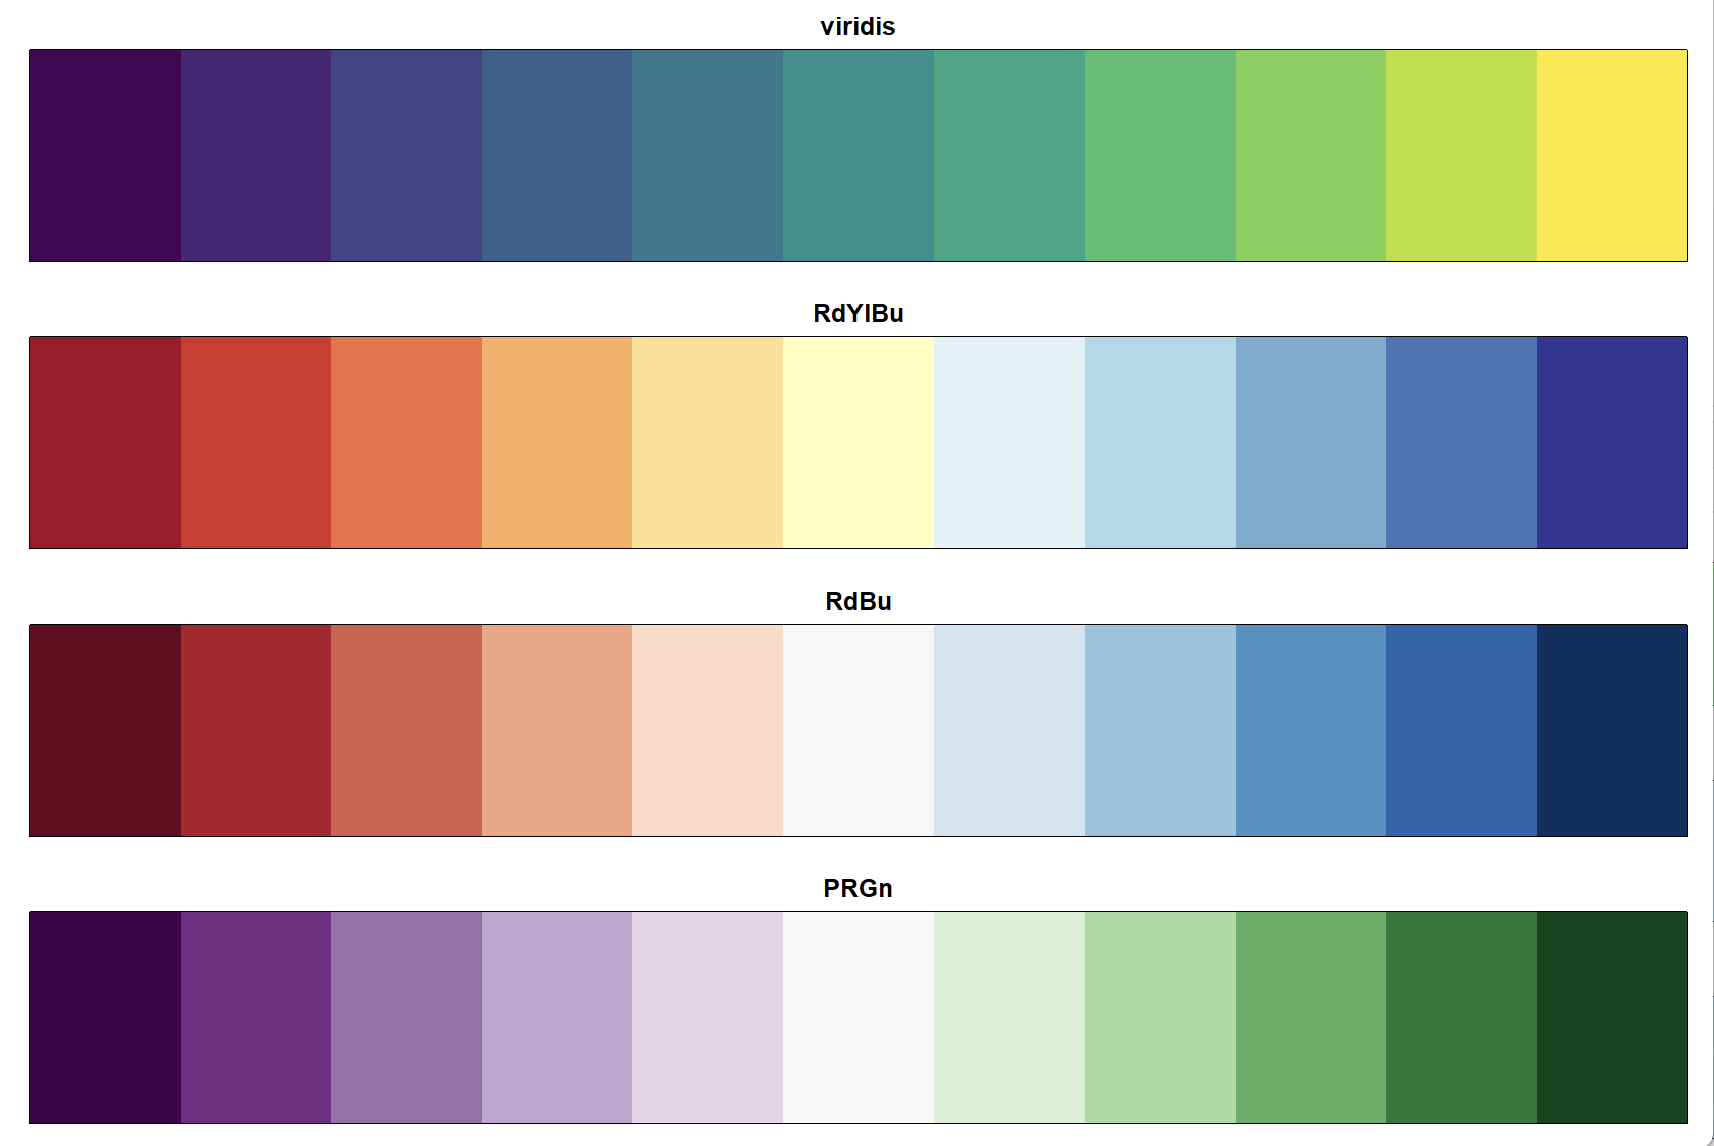
\includegraphics[width=0.6\textwidth]{farbpaletten.png}
	\caption{Übersicht der vier verwendeten Farbpaletten, erzeugt mit den R-Paketen \texttt{RColorBrewer} \cite{HarrowerBrewer2003} und \texttt{viridis} \cite{Viridis}.}
	\label{fig:farbpaletten}
\end{figure}


\begin{table}[H]
	\centering
	\small
	\vspace{0.2cm}
	\begin{tabularx}{\textwidth}{l l X}
		\toprule
		\textbf{Palette} & \textbf{Typ} & \textbf{Einsatzzweck und Begründung} \\
		\midrule
		\texttt{RdYlBu} & Divergierend & Bietet durch das helle, gelbe Zentrum einen neutralen Mittelpunkt für zweiseitige Abweichungen. Die Unterscheidung der äußeren Maxima mit Rot und Blau sind bewusst mit annähernd gleicher visueller Intensität gewählt und gut differenzierbar für Menschen mit einer Rot-Grün-Schwäche. \\
		\addlinespace
		\texttt{RdBu} & Divergierend & Ein klassisches, in der Genexpressionsanalyse bewährtes Farbschema, das maximale Kontraste liefert. Da die Palette mit Rot, Weiß und Blau auf Grünanteile verzichtet, ist sie zudem für Personen mit Rot-Grün-Schwäche gut differenzierbar. \\
		\addlinespace
		\texttt{PRGn} & Divergierend & Dient als kontrastreiche Alternative zu traditionellen Skalen. Da die Unterscheidung von Violett und Grün nicht auf der Rot-Grün-Achse, sondern zusätzlich über die Blau-Gelb-Wahrnehmung erfolgt, ist die Kombination für Personen mit der deutlich häufigeren Rot-Grün-Sehschwäche gut differenzierbar. \\
		\addlinespace
		\texttt{viridis} & Sequentiell & Zeichnet sich durch einen gleichmäßigen, monoton steigenden Verlauf der Luminanz (Helligkeit) aus. Die visuelle Information bleibt auch bei Konvertierung in Graustufen oder Schwarz-Weiß-Druck vollständig erhalten. \\
		\bottomrule
	\end{tabularx}
	\caption{Vergleich der implementierten Farbpaletten für die Heatmap-Generierung.}
	\label{tab:farbpaletten}
\end{table}

Die drei divergierenden Paletten \texttt{RdYlBu}, \texttt{RdBu} und \texttt{PRGn} sind dabei gezielt so konstruiert, dass ihre beiden äußeren Farbwerte eine annähernd gleiche Sättigung und Helligkeit aufweisen \cite{HarrowerBrewer2003}. Dadurch wird vermieden, dass eine der beiden Richtungen einer Abweichung, etwa Über- oder Unterexpression eines Gens, allein aufgrund der Farbwahl visuell stärker gewichtet oder als bedeutsamer wahrgenommen wird als die andere.

Für die Heatmap wird von den Farbpaletten jeweils der vollständige, elfstufige Verlauf verwendet, bei der farblichen Kennzeichnung der Labels im Dendrogramm ergibt sich hingegen eine andere Anforderung. Während für die Heatmap eine sequentielle bzw. divergierende Ordnung kontinuierlicher Expressionswerte abgebildet werden muss, ist für die qualitative Kennzeichnung der Patienten eine unbekannte Anzahl von diskreten Gruppen, ohne natürliche Rangfolge nötig \cite{HarrowerBrewer2003}. Um ein harmonisches Bild zu erzeugen orientiert sich die Farbgebung des Dendrogramms zwar an den Farbpaletten der Heatmap, verwendet jedoch nur neun der elf Farbabstufungen, da die mittleren hellen Töne oftmals nicht zuverlässig erkennbar und unterscheidbar sind. 

Da es aber durchaus vorkommen kann, dass die Anzahl der zu kennzeichnenden Labels diese neun Farben übersteigt, existiert für diesen Fall ein sogenannter \texttt{default\_colors}-Vektor. Er enthält 20 gut unterscheidbare Farben. Dabei wurde auf folgende Kriterien geachtet. Es wurden kaum stark leuchtende Neonfarben verwendet, da diese bei längerer Betrachtung zu visueller Ermüdung führen und unangemessen stark hervortreten würden \cite{Tufte1983}. Pastelltöne und schwer unterscheidbare Farben wurden ebenfalls ausgeschlossen, da sie auf dem hellen GUI-Hintergrund zu wenig Kontrast bieten würden. Zusätzlich wurde die Reihenfolge der Farben in der Liste so angepasst, dass stets ein deutlicher Farbabstand zwischen zwei aufeinanderfolgenden Labels besteht, um auch bei direkt benachbarter Vergabe eine gute Unterscheidbarkeit zu gewährleisten.

\begin{figure}[H]
	\centering
	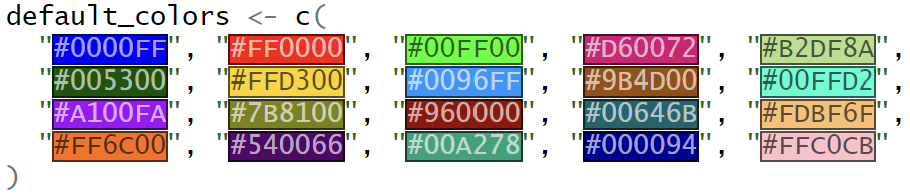
\includegraphics[width=0.6\textwidth]{default_colors.png}
	\caption{Übersicht der 20 Farben des \texttt{default\_colors}-Vektors.}
	\label{fig:default-colors}
\end{figure}

\subsubsection{Schwierigkeiten}
Gut unterscheidbare Farbpaletten zu finden, die alle Anforderungen, vor allem die der Verzerrungsfreiheit erfüllen, aber auch die \texttt{default\_colors} gut unterscheidbar auszuwählen, war nicht immer leicht. Die größten fachlichen Schwierigkeiten in diesem Projekt hat mir allerdings die farbliche Darstellung des Dendrogramms bereitet. Da die Linien dort sehr dünn auf weißem Hintergrund dargestellt werden, waren helle Farben aus den ausgewählten Farbpaletten häufig nicht gut erkennbar. Deshalb mussten die Abstufungen für das Dendrogramm entsprechend angepasst werden. Dieses Problem wurde leider auch erst vergleichsweise spät im Projektverlauf sichtbar, da die konzipierte Farbgebung erst spät ins Dendrogramm eingebaut wurde. Mit dem letztendlich erzielten Ergebnis bin ich zwar zufrieden, denke aber, dass sich eine noch feinere Abstimmung hätte erarbeiten lassen, wenn die getroffenen Absprachen von Beginn an konsequenter und fristgerecht eingehalten worden wären.


\begin{table}[H]
	\begin{tabular}{l|l|l}
		Aufgabe                       & Zuständig & Arbeitsaufwand \\ 
		\hline
		Recherche Farbdarstellungen             & Johanna   & 7 Stunden               \\
		Testen verschiedener Farbtabellen     & Johanna   & 2 Stunden               \\ 
		Datenfluss-Modell erstellt     	& Johanna   & 1 Stunden               \\
		Zusammenstellen der default-colors             & Johanna   & 1,5 Stunden      \\ 
		Grundlagen Kapitel Biologie verfasst              & Johanna   & 10 Stunden               \\ 
		Grundlagen Kapitel Medizin  verfasst              & Johanna   & 8 Stunden               \\ 
		Ausarbeitung Farben verfasst              & Johanna   & 8 Stunden               \\
		Vorbereitung Präsentation              & Johanna   & 5 Stunden               \\
		Kommunikation zwischen den Teams   & Johanna   & 4 Stunden      \\ 
		Meetings mit Adrika                & Johanna   & 3 Stunden    \\ 
		Absprachen mit Visualisierungsteam                & Johanna   & 6 Stunden    \\ 
		Gruppenmeetings                & Johanna   & 19,5 Stunden    \\ 
	\end{tabular}
\end{table}

\newpage

\bibliographystyle{plain} % Styles include plain, unsrt, alpha, apalike
\bibliography{bibliography}

\end{document}
